
%% bare_jrnl.tex
%% V1.4b
%% 2015/08/26
%% by Michael Shell
%% see http://www.michaelshell.org/
%% for current contact information.
%%
%% This is a skeleton file demonstrating the use of IEEEtran.cls
%% (requires IEEEtran.cls version 1.8b or later) with an IEEE
%% journal paper.
%%
%% Support sites:
%% http://www.michaelshell.org/tex/ieeetran/
%% http://www.ctan.org/pkg/ieeetran
%% and
%% http://www.ieee.org/

%%*************************************************************************
%% Legal Notice:
%% This code is offered as-is without any warranty either expressed or
%% implied; without even the implied warranty of MERCHANTABILITY or
%% FITNESS FOR A PARTICULAR PURPOSE! 
%% User assumes all risk.
%% In no event shall the IEEE or any contributor to this code be liable for
%% any damages or losses, including, but not limited to, incidental,
%% consequential, or any other damages, resulting from the use or misuse
%% of any information contained here.
%%
%% All comments are the opinions of their respective authors and are not
%% necessarily endorsed by the IEEE.
%%
%% This work is distributed under the LaTeX Project Public License (LPPL)
%% ( http://www.latex-project.org/ ) version 1.3, and may be freely used,
%% distributed and modified. A copy of the LPPL, version 1.3, is included
%% in the base LaTeX documentation of all distributions of LaTeX released
%% 2003/12/01 or later.
%% Retain all contribution notices and credits.
%% ** Modified files should be clearly indicated as such, including  **
%% ** renaming them and changing author support contact information. **
%%*************************************************************************


% *** Authors should verify (and, if needed, correct) their LaTeX system  ***
% *** with the testflow diagnostic prior to trusting their LaTeX platform ***
% *** with production work. The IEEE's font choices and paper sizes can   ***
% *** trigger bugs that do not appear when using other class files.       ***                          ***
% The testflow support page is at:
% http://www.michaelshell.org/tex/testflow/



\documentclass[journal]{IEEEtran}
%
% If IEEEtran.cls has not been installed into the LaTeX system files,
% manually specify the path to it like:
% \documentclass[journal]{../sty/IEEEtran}





% Some very useful LaTeX packages include:
% (uncomment the ones you want to load)


% *** MISC UTILITY PACKAGES ***
%
%\usepackage{ifpdf}
% Heiko Oberdiek's ifpdf.sty is very useful if you need conditional
% compilation based on whether the output is pdf or dvi.
% usage:
% \ifpdf
%   % pdf code
% \else
%   % dvi code
% \fi
% The latest version of ifpdf.sty can be obtained from:
% http://www.ctan.org/pkg/ifpdf
% Also, note that IEEEtran.cls V1.7 and later provides a builtin
% \ifCLASSINFOpdf conditional that works the same way.
% When switching from latex to pdflatex and vice-versa, the compiler may
% have to be run twice to clear warning/error messages.

\usepackage{algorithm,algpseudocode}
\usepackage{comment}
\usepackage{multirow}




% *** CITATION PACKAGES ***
%
%\usepackage{cite}
% cite.sty was written by Donald Arseneau
% V1.6 and later of IEEEtran pre-defines the format of the cite.sty package
% \cite{} output to follow that of the IEEE. Loading the cite package will
% result in citation numbers being automatically sorted and properly
% "compressed/ranged". e.g., [1], [9], [2], [7], [5], [6] without using
% cite.sty will become [1], [2], [5]--[7], [9] using cite.sty. cite.sty's
% \cite will automatically add leading space, if needed. Use cite.sty's
% noadjust option (cite.sty V3.8 and later) if you want to turn this off
% such as if a citation ever needs to be enclosed in parenthesis.
% cite.sty is already installed on most LaTeX systems. Be sure and use
% version 5.0 (2009-03-20) and later if using hyperref.sty.
% The latest version can be obtained at:
% http://www.ctan.org/pkg/cite
% The documentation is contained in the cite.sty file itself.

%\usepackage[maxbibnames=4]{biblatex}




% *** GRAPHICS RELATED PACKAGES ***
%
\ifCLASSINFOpdf
  % \usepackage[pdftex]{graphicx}
  % declare the path(s) where your graphic files are
  % \graphicspath{{../pdf/}{../jpeg/}}
  % and their extensions so you won't have to specify these with
  % every instance of \includegraphics
  % \DeclareGraphicsExtensions{.pdf,.jpeg,.png}
\else
  % or other class option (dvipsone, dvipdf, if not using dvips). graphicx
  % will default to the driver specified in the system graphics.cfg if no
  % driver is specified.
  % \usepackage[dvips]{graphicx}
  % declare the path(s) where your graphic files are
  % \graphicspath{{../eps/}}
  % and their extensions so you won't have to specify these with
  % every instance of \includegraphics
  % \DeclareGraphicsExtensions{.eps}
\fi
% graphicx was written by David Carlisle and Sebastian Rahtz. It is
% required if you want graphics, photos, etc. graphicx.sty is already
% installed on most LaTeX systems. The latest version and documentation
% can be obtained at: 
% http://www.ctan.org/pkg/graphicx
% Another good source of documentation is "Using Imported Graphics in
% LaTeX2e" by Keith Reckdahl which can be found at:
% http://www.ctan.org/pkg/epslatex
%
% latex, and pdflatex in dvi mode, support graphics in encapsulated
% postscript (.eps) format. pdflatex in pdf mode supports graphics
% in .pdf, .jpeg, .png and .mps (metapost) formats. Users should ensure
% that all non-photo figures use a vector format (.eps, .pdf, .mps) and
% not a bitmapped formats (.jpeg, .png). The IEEE frowns on bitmapped formats
% which can result in "jaggedy"/blurry rendering of lines and letters as
% well as large increases in file sizes.
%
% You can find documentation about the pdfTeX application at:
% http://www.tug.org/applications/pdftex

\usepackage{caption}
\usepackage{color}
\usepackage{adjustbox}



% *** MATH PACKAGES ***
%
\usepackage{amsmath}
% A popular package from the American Mathematical Society that provides
% many useful and powerful commands for dealing with mathematics.
%
% Note that the amsmath package sets \interdisplaylinepenalty to 10000
% thus preventing page breaks from occurring within multiline equations. Use:
%\interdisplaylinepenalty=2500
% after loading amsmath to restore such page breaks as IEEEtran.cls normally
% does. amsmath.sty is already installed on most LaTeX systems. The latest
% version and documentation can be obtained at:
% http://www.ctan.org/pkg/amsmath

\usepackage{mathtools} %tools for mathematical writing
\usepackage{amssymb}




% *** SPECIALIZED LIST PACKAGES ***
%
%\usepackage{algorithmic}
% algorithmic.sty was written by Peter Williams and Rogerio Brito.
% This package provides an algorithmic environment fo describing algorithms.
% You can use the algorithmic environment in-text or within a figure
% environment to provide for a floating algorithm. Do NOT use the algorithm
% floating environment provided by algorithm.sty (by the same authors) or
% algorithm2e.sty (by Christophe Fiorio) as the IEEE does not use dedicated
% algorithm float types and packages that provide these will not provide
% correct IEEE style captions. The latest version and documentation of
% algorithmic.sty can be obtained at:
% http://www.ctan.org/pkg/algorithms
% Also of interest may be the (relatively newer and more customizable)
% algorithmicx.sty package by Szasz Janos:
% http://www.ctan.org/pkg/algorithmicx




% *** ALIGNMENT PACKAGES ***
%
%\usepackage{array}
% Frank Mittelbach's and David Carlisle's array.sty patches and improves
% the standard LaTeX2e array and tabular environments to provide better
% appearance and additional user controls. As the default LaTeX2e table
% generation code is lacking to the point of almost being broken with
% respect to the quality of the end results, all users are strongly
% advised to use an enhanced (at the very least that provided by array.sty)
% set of table tools. array.sty is already installed on most systems. The
% latest version and documentation can be obtained at:
% http://www.ctan.org/pkg/array


% IEEEtran contains the IEEEeqnarray family of commands that can be used to
% generate multiline equations as well as matrices, tables, etc., of high
% quality.




% *** SUBFIGURE PACKAGES ***
%\ifCLASSOPTIONcompsoc
%  \usepackage[caption=false,font=normalsize,labelfont=sf,textfont=sf]{subfig}
%\else
%  \usepackage[caption=false,font=footnotesize]{subfig}
%\fi
% subfig.sty, written by Steven Douglas Cochran, is the modern replacement
% for subfigure.sty, the latter of which is no longer maintained and is
% incompatible with some LaTeX packages including fixltx2e. However,
% subfig.sty requires and automatically loads Axel Sommerfeldt's caption.sty
% which will override IEEEtran.cls' handling of captions and this will result
% in non-IEEE style figure/table captions. To prevent this problem, be sure
% and invoke subfig.sty's "caption=false" package option (available since
% subfig.sty version 1.3, 2005/06/28) as this is will preserve IEEEtran.cls
% handling of captions.
% Note that the Computer Society format requires a larger sans serif font
% than the serif footnote size font used in traditional IEEE formatting
% and thus the need to invoke different subfig.sty package options depending
% on whether compsoc mode has been enabled.
%
% The latest version and documentation of subfig.sty can be obtained at:
% http://www.ctan.org/pkg/subfig
\usepackage{subfig}




% *** FLOAT PACKAGES ***
%
%\usepackage{fixltx2e}
% fixltx2e, the successor to the earlier fix2col.sty, was written by
% Frank Mittelbach and David Carlisle. This package corrects a few problems
% in the LaTeX2e kernel, the most notable of which is that in current
% LaTeX2e releases, the ordering of single and double column floats is not
% guaranteed to be preserved. Thus, an unpatched LaTeX2e can allow a
% single column figure to be placed prior to an earlier double column
% figure.
% Be aware that LaTeX2e kernels dated 2015 and later have fixltx2e.sty's
% corrections already built into the system in which case a warning will
% be issued if an attempt is made to load fixltx2e.sty as it is no longer
% needed.
% The latest version and documentation can be found at:
% http://www.ctan.org/pkg/fixltx2e
\usepackage{float}


%\usepackage{stfloats}
% stfloats.sty was written by Sigitas Tolusis. This package gives LaTeX2e
% the ability to do double column floats at the bottom of the page as well
% as the top. (e.g., "\begin{figure*}[!b]" is not normally possible in
% LaTeX2e). It also provides a command:
%\fnbelowfloat
% to enable the placement of footnotes below bottom floats (the standard
% LaTeX2e kernel puts them above bottom floats). This is an invasive package
% which rewrites many portions of the LaTeX2e float routines. It may not work
% with other packages that modify the LaTeX2e float routines. The latest
% version and documentation can be obtained at:
% http://www.ctan.org/pkg/stfloats
% Do not use the stfloats baselinefloat ability as the IEEE does not allow
% \baselineskip to stretch. Authors submitting work to the IEEE should note
% that the IEEE rarely uses double column equations and that authors should try
% to avoid such use. Do not be tempted to use the cuted.sty or midfloat.sty
% packages (also by Sigitas Tolusis) as the IEEE does not format its papers in
% such ways.
% Do not attempt to use stfloats with fixltx2e as they are incompatible.
% Instead, use Morten Hogholm'a dblfloatfix which combines the features
% of both fixltx2e and stfloats:
%
% \usepackage{dblfloatfix}
% The latest version can be found at:
% http://www.ctan.org/pkg/dblfloatfix




%\ifCLASSOPTIONcaptionsoff
%  \usepackage[nomarkers]{endfloat}
% \let\MYoriglatexcaption\caption
% \renewcommand{\caption}[2][\relax]{\MYoriglatexcaption[#2]{#2}}
%\fi
% endfloat.sty was written by James Darrell McCauley, Jeff Goldberg and 
% Axel Sommerfeldt. This package may be useful when used in conjunction with 
% IEEEtran.cls'  captionsoff option. Some IEEE journals/societies require that
% submissions have lists of figures/tables at the end of the paper and that
% figures/tables without any captions are placed on a page by themselves at
% the end of the document. If needed, the draftcls IEEEtran class option or
% \CLASSINPUTbaselinestretch interface can be used to increase the line
% spacing as well. Be sure and use the nomarkers option of endfloat to
% prevent endfloat from "marking" where the figures would have been placed
% in the text. The two hack lines of code above are a slight modification of
% that suggested by in the endfloat docs (section 8.4.1) to ensure that
% the full captions always appear in the list of figures/tables - even if
% the user used the short optional argument of \caption[]{}.
% IEEE papers do not typically make use of \caption[]'s optional argument,
% so this should not be an issue. A similar trick can be used to disable
% captions of packages such as subfig.sty that lack options to turn off
% the subcaptions:
% For subfig.sty:
% \let\MYorigsubfloat\subfloat
% \renewcommand{\subfloat}[2][\relax]{\MYorigsubfloat[]{#2}}
% However, the above trick will not work if both optional arguments of
% the \subfloat command are used. Furthermore, there needs to be a
% description of each subfigure *somewhere* and endfloat does not add
% subfigure captions to its list of figures. Thus, the best approach is to
% avoid the use of subfigure captions (many IEEE journals avoid them anyway)
% and instead reference/explain all the subfigures within the main caption.
% The latest version of endfloat.sty and its documentation can obtained at:
% http://www.ctan.org/pkg/endfloat
%
% The IEEEtran \ifCLASSOPTIONcaptionsoff conditional can also be used
% later in the document, say, to conditionally put the References on a 
% page by themselves.




% *** PDF, URL AND HYPERLINK PACKAGES ***
%
%\usepackage{url}
% url.sty was written by Donald Arseneau. It provides better support for
% handling and breaking URLs. url.sty is already installed on most LaTeX
% systems. The latest version and documentation can be obtained at:
% http://www.ctan.org/pkg/url
% Basically, \url{my_url_here}.

\usepackage{hyperref} % For hyperlinks in the PDF

\hypersetup{
    colorlinks=true,
    linkcolor=black,
    filecolor=magenta,      
    urlcolor=blue,
    citecolor=black
}




% *** Do not adjust lengths that control margins, column widths, etc. ***
% *** Do not use packages that alter fonts (such as pslatex).         ***
% There should be no need to do such things with IEEEtran.cls V1.6 and later.
% (Unless specifically asked to do so by the journal or conference you plan
% to submit to, of course. )


% correct bad hyphenation here
\hyphenation{op-tical net-works semi-conduc-tor}


\begin{document}
%
% paper title
% Titles are generally capitalized except for words such as a, an, and, as,
% at, but, by, for, in, nor, of, on, or, the, to and up, which are usually
% not capitalized unless they are the first or last word of the title.
% Linebreaks \\ can be used within to get better formatting as desired.
% Do not put math or special symbols in the title.

\title{Automatic model selection for neural networks}
%
%
% author names and IEEE memberships
% note positions of commas and nonbreaking spaces ( ~ ) LaTeX will not break
% a structure at a ~ so this keeps an author's name from being broken across
% two lines.
% use \thanks{} to gain access to the first footnote area
% a separate \thanks must be used for each paragraph as LaTeX2e's \thanks
% was not built to handle multiple paragraphs
%

\begin{comment}
\author{David Laredo% <-this % stops a space
\thanks{D. Laredo is with the Department of Mechanical Engineering, University of California, Merced,
CA, 95340 USA e-mail: dlaredorazo@ucmerced.edu.}}% <-this % stops a space
\end{comment}

\author{David Laredo, Jian-Qiao Sun, Yulin Qin% <-this % stops a space
\thanks{All the authors are affiliated with the Department of Mechanical Engineering, University of California, Merced,
CA, 95340 USA e-mail: dlaredorazo@ucmerced.edu.}}% <-this % stops a space

% note the % following the last \IEEEmembership and also \thanks - 
% these prevent an unwanted space from occurring between the last author name
% and the end of the author line. i.e., if you had this:
% 
% \author{....lastname \thanks{...} \thanks{...} }
%                     ^------------^------------^----Do not want these spaces!
%
% a space would be appended to the last name and could cause every name on that
% line to be shifted left slightly. This is one of those "LaTeX things". For
% instance, "\textbf{A} \textbf{B}" will typeset as "A B" not "AB". To get
% "AB" then you have to do: "\textbf{A}\textbf{B}"
% \thanks is no different in this regard, so shield the last } of each \thanks
% that ends a line with a % and do not let a space in before the next \thanks.
% Spaces after \IEEEmembership other than the last one are OK (and needed) as
% you are supposed to have spaces between the names. For what it is worth,
% this is a minor point as most people would not even notice if the said evil
% space somehow managed to creep in.



% The paper headers
\markboth{Journal of \LaTeX\ Class Files,~Vol.~14, No.~8, August~2015}%
{Shell \MakeLowercase{\textit{et al.}}: Bare Demo of IEEEtran.cls for IEEE Journals}
% The only time the second header will appear is for the odd numbered pages
% after the title page when using the twoside option.
% 
% *** Note that you probably will NOT want to include the author's ***
% *** name in the headers of peer review papers.                   ***
% You can use \ifCLASSOPTIONpeerreview for conditional compilation here if
% you desire.




% If you want to put a publisher's ID mark on the page you can do it like
% this:
%\IEEEpubid{0000--0000/00\$00.00~\copyright~2015 IEEE}
% Remember, if you use this you must call \IEEEpubidadjcol in the second
% column for its text to clear the IEEEpubid mark.



% use for special paper notices
%\IEEEspecialpapernotice{(Invited Paper)}




% make the title area
\maketitle

% As a general rule, do not put math, special symbols or citations
% in the abstract or keywords.
\begin{abstract}
Neural networks and deep learning are changing the way that artificial intelligence is being done. Efficiently choosing a suitable model (including hyperparameters) for a specific problem is a time-consuming task. Choosing among the many different combinations of neural networks available gives rise to a staggering number of possible alternatives overall. Here we address this problem by proposing a fully automated framework for efficiently selecting a neural network model given a specific problem (whether it is classification or regression). Our proposal focuses on a distributed decision-making algorithm for keeping the most promising models among a pool of possible models for one of the major neural network architectures, Multi-Layer Perceptrons (MLPs). This work develops Automatic Model Selection (AMS), a modified micro genetic algorithm that automatically and efficiently finds the most suitable neural network model for a given dataset. Our contributions include: a simple list based encoding for neural networks as genotypes in an evolutionary algorithm, new crossover and mutation operators, the introduction of a fitness function that considers both, the accuracy of the model and its complexity and a method to measure the similarity between two neural networks. Our evaluation on two different datasets show that AMS effectively finds suitable neural network models while being efficient in terms of the computational burden, our results are compared against other state of the art methods such as Auto-Keras and AutoML.
\end{abstract}

% Note that keywords are not normally used for peerreview papers.
\begin{IEEEkeywords}
artificial neural networks, model selection, hyperparameter tuning, distributed computing, evolutionary algorithms.
\end{IEEEkeywords}






% For peer review papers, you can put extra information on the cover
% page as needed:
% \ifCLASSOPTIONpeerreview
% \begin{center} \bfseries EDICS Category: 3-BBND \end{center}
% \fi
%
% For peerreview papers, this IEEEtran command inserts a page break and
% creates the second title. It will be ignored for other modes.
%\IEEEpeerreviewmaketitle



\section{Introduction}
% The very first letter is a 2 line initial drop letter followed
% by the rest of the first word in caps.
% 
% form to use if the first word consists of a single letter:
% \IEEEPARstart{A}{demo} file is ....
% 
% form to use if you need the single drop letter followed by
% normal text (unknown if ever used by the IEEE):
% \IEEEPARstart{A}{}demo file is ....
% 
% Some journals put the first two words in caps:
% \IEEEPARstart{T}{his demo} file is ....
% 
% Here we have the typical use of a "T" for an initial drop letter
% and "HIS" in caps to complete the first word.
\IEEEPARstart{M}{achine} learning studies algorithms that improve themselves through experience. Given the large amounts of data currently available in many fields such as engineering, biomedical, finance, etc, and the increasingly computing power available machine learning is now practiced by people with very diverse backgrounds. Increasingly, users of machine learning tools are non-experts who require off-the-shelf solutions. Automated Machine Learning (AutoML) is the field of machine learning devoted to developing algorithms and solutions to enable people with limited machine learning background knowledge to use use machine learning models easily. Tools like WEKA \cite{Hall2009}, PyBrain \cite{Schaul2010} or MLLib \cite{mlib2017} follow this paradigm. Nevertheless, the user still needs to make some choices which not may be obvious or intuitive (selecting a learning algorithm, hyperparameters, features, etc) thus leading to the selection of non optimal models.

Recently, deep learning models (CNN, RNN, Deep NN) have gained a lot of attention due their improved efficiency on complex learning problems and their flexibility and generality for solving a large number of problems such as: regression, classification, natural language processing, recommendation systems, etc. Furthermore, there are a lot software libraries which makes their implementation easier. TensorFlow \cite{TensorFlow2015}, Keras \cite{keras2015}, Caffe \cite{caffe2014} and CNTK \cite{cntk2016} are some examples of such libraries. Despite the availability of such libraries and tools, the task of picking the right neural network model  and its hyperparameters is usually complex and iterative in nature specially among non computer scientist.

Usually, the process of selecting a suitable machine learning model for a particular problem is done in an iterative manner. First, an input dataset must be transformed from a domain specific format to features which are predictive of the field of interest, once features have been engineered users must pick a learning setting appropriate to their problem, e.g. regression, classification or recommendation. Next users must pick an appropriate model, such as support vector machines (SVM), logistic regression or any flavor of neural networks (NNs). Each model family has a number of hyperparameters, such as regularization degree, learning rate, number of neurons, etc, and each of these must be tuned to achieve optimal results. Finally, users must pick a software package that can train their model, configure one or more machines to execute the training and evaluate the model's quality. It can be challenging to make the right choice when faced with so many degrees of freedom, leaving many users to select a model based on intuition or randomness and/or leave hyperparameters set to default, this approach will usually yield suboptimal results.

This suggests a natural challenge for machine learning: given a dataset, to automatically and simultaneously chose a learning algorithm and set its hyperparameters to optimize performance. As mentioned in \cite{Hall2009} the combined space of learning algorithm and hyperparemeters is very challenging to search: the response function is noisy and the space is high dimensional involving both, categorical and continuous choices and containing hierarchical dependencies (e.g. hyperparameters of the algorithm are only meaningful if that algorithm is chosen). Thus, identifying a high quality model is typically costly (in the sense that entails a lot of computational effort) and time consuming.

To address this challenges we propose Automatic Model Selection (AMS) a flexible and scalable method to automate the process of selecting artificial neural network models. The key contributions of this paper include: 1) a simple, list based encoding of neural networks as genotypes for evolutionary computation algorithms, 2) new crossover and mutation operators to generate valid neural networks models from an evolutionary algorithm, 3) the introduction of a fitness function that considers both, the accuracy of the model and its complexity and 3) a method for measuring the similarity between two neural networks. All these components together form a new method based on an evolutionary algorithm, which we call AMS, and that can be used to find an optimal neural network architecture for a given dataset.

The remainder of this paper is organized as follows: Section \ref{sec:model_selection} formally introduces the model selection problem. The related work is briefly reviewed in Section \ref{sec:literature_review}. The AMS algorithm and all of its components are described in detail in Section \ref{sec:auto_nn}, experiments to test the algorithm and comparison against other state of the art methods are presented in Section \ref{sec:evaluation}. Conclusions and future work are discussed in Section \ref{sec:conclusions}.

%----------------------------------------------------------------------------------------
%	Model selection
%----------------------------------------------------------------------------------------

\section{Problem Statement}
\label{sec:model_selection}

In this section we mathematically define the general neural network architecture search problem. Consider a dataset $\mathcal{D}$ made up of training points $d_i = (\mathbf{x_i}, \mathbf{y_i}) \in \mathcal{X} \times \mathcal{Y}$ where $\mathcal{X}$ is the set of data points and $\mathcal{Y}$ is the set of labels. Furthermore, lets split the dataset into training set $D_t$, cross validation set $D_v$, and test set $D_e$. Given a neural network architecture search space $\mathcal{F}$ the performance of a neural network architecture $f \in \mathcal{F}$ on trained on $\mathcal{D}_t$ and validated with  $\mathcal{D}_v$ is defined as:

\begin{equation}
p = Per(f(D_t); D_v),
\label{eq:nn_cost}
\end{equation}

where $Perf(.)$ can be any standard or custom cost metric, e.g. accuracy, precision, mean squared error, etc.  Commonly used performance indicators can be found in Table \ref{table:performance_metrics}. 

Finding a neural network $f^* \in \mathcal{F}$ that achieves a good performance has been explored in \cite{Jin2018, Real2018} among others. While this task alone is challenging, usually the efficiency of $f^*$ is not measured. Indeed, it turns out that there can be several candidate models that can attain similar performance with improved efficiency. By efficiency we mean, in practical terms, how fast is to train $f^*$ as compared to other possible solutions. 

In this paper we aim to achive neural network models $f^*$ that not only exhibit good performance in $\mathcal{D}$ as measured by $p$ but also achieves such performance using a simple structure, which directly translates to improved efficiency of the model. To measure the complexity of the architecture we make use of the number of trainable parameters $w(f)$ of the neural network, we will also refer to $w(f)$ as the ``size'' of the neural network.

The problem of finding an neural network $f$ that achieves both a good performance on the dataset $\mathcal{D}$ with a simple model can be mathematically stated as the following multiobjective optimization problem:

\begin{equation}
	\begin{aligned}
	f^* = \underset{f \in \mathcal{F}}{\text{argmin}}
	& \quad (p(f), w(f))\\
	\end{aligned}
	\label{eq:model_selection_eq}
\end{equation}

In this paper we develop an algorithm to efficiently solve Eq. \ref{eq:model_selection_eq}.





\begin{comment}
\section{The CASH problem}
\label{sec:model_selection}

In this section we introduce and formally describe the model selection problem, our description borrows the definitions given in \cite{Thornton2013}. For the sake of simplicity, for this work we only consider supervised learning problems, i.e. learning a function $f: \mathcal{X} \mapsto \mathcal{Y}$ with finite $\mathcal{Y}$ labels. A learning algorithm $A$ maps a set $\{d_1, \ldots, d_n\}$ of training data points $d_i = (\mathbf{x_i}, \mathbf{y_i}) \in \mathcal{X} \times \mathcal{Y}$ to such a function $f$. Most learning algorithms $A$ further expose hyperparameters $\lambda \in \mathbf{\Lambda}$, which change the way the learning algorithm $A_{\lambda}$ works. One example of hyperparameters is the number of neurons in a hidden layer of an artificial neural network (ANN), another common example is the learning rate $\alpha$ of a neural network. These hyperparameters are typically optmized in an ``outer loop'' that evaluates the performance of each hyperparameter configuration using cross-validation \cite{alpaydin2010}.

\subsection{Model selection}

Given a set of learning algorithms $\mathcal{A}$ and a limited amount of training data $\mathcal{D} = \{ (\mathbf{x_1}, \mathbf{y_1}, \ldots \mathbf{x_n}, \mathbf{y_n}) \}$, the goal of model selection is to determine the algorithm $A^* \in \mathcal{A}$ with optimal generalization performance. Generalization performance is estimated by splitting $\mathcal{D}$ into disjoint training and validation sets $\mathcal{D}_{t}$ and $\mathcal{D}_{v}$ respectively, learning function $f$ by applying $A^*$ to $\mathcal{D}_{t}$, and evaluating the predictive performance of this function on $\mathcal{D}_{v}$. Using $k$-fold validation, which splits the data into $k$ equal sized cross validation partitions $ \mathcal{D}^{1}_{v}, \ldots,  \mathcal{D}^{k}_{v}$ and training partition $ \mathcal{D}^{i}_{t} =  D \backslash D^{i}_{v}$ for $i = 1, \ldots, k$ the model selection problem is defined as:

\begin{equation}
A^* \in \underset{A \in \mathcal{A}}{\operatorname{argmin}} \frac{1}{k} \sum_{i=1}^{k} \mathcal{L} \left( A, \mathcal{D}^{i}_{t},  \mathcal{D}^{i}_{v} \right),
\end{equation}

where $ \mathcal{L} \left( A, \mathcal{D}^{i}_{t},  \mathcal{D}^{i}_{v} \right) $ is the loss achieved by $A$ when trained on $\mathcal{D}^{i}_{t}$ and evaluated on $\mathcal{D}^{i}_{v}$. 

\subsection{Hyperparameter optimization}

The problem of optimizing the hyperparameters $\lambda \in \mathbf{\Lambda}$ of a given learning algorithm $A$ is conceptually similar to that of model selection. Some key differences are that hyperparameters are often continuous, hyperparameter spaces are often high dimensional, and that correlation structure between different hyperparameter settings $\lambda_1,\lambda_2 \in \mathbf{\Lambda} $ can be exploited. Given $n$ hyperparameters $\lambda_1, \ldots, \lambda_n$ with domains $\Lambda_1, \ldots, \Lambda_n$ , the hyperparameter space $\mathbf{\Lambda}$ is a subset of the crossproduct of these domains: $\mathbf{\Lambda} \subset \Lambda_1 \times \ldots \times \Lambda_n$. This subset is often strict, such as when certain settings of one hyperparameter render other hyperparameters inactive. For example, the parameters determining the specifics of the third layer of a deep neural network are not relevant if the network depth is set to one or two. The hyperparameter optimization problem can be written as:

\begin{equation}
\lambda^* \in \underset{\lambda \in \mathbf{\Lambda}}{\operatorname{argmin}} \frac{1}{k} \sum_{i=1}^{k} \mathcal{L} \left( A_{\lambda}, \mathcal{D}^{i}_{t},  \mathcal{D}^{i}_{v} \right),
\end{equation}

In this study we consider the more general combined algorithm selection and hyperparameter optimization (CASH). That is we intend to optimize both problems at the same time. Given a set of algorithms $\mathbb{A} = \left\lbrace A^{(1)}, \ldots, A^{(k)} \right\rbrace$ with associated hyperparameter spaces $\mathbf{\Lambda}^{(1)}, \ldots \mathbf{\Lambda}^{(k)}$, the CASH problem is the defined as computing

\begin{equation}
A^* \lambda^* \in \underset{A^{(j)} \in \mathcal{A}, \lambda \in \mathbf{\Lambda}^{(j)}}{\operatorname{argmin}} \frac{1}{k} \sum_{i=1}^{k} \mathcal{L} \left( A_{\lambda}^{(j)}, \mathcal{D}^{i}_{t},  \mathcal{D}^{i}_{v} \right).
\end{equation}

For our particular application we consider $\mathcal{A}$ as the set of all possible fully connected neural network, also known as multi-layer perceptron (MLP), model configurations, i.e. number of layers and number of neurons per layer, and $\Lambda$ as the set of all possible hyperparameters for an MLP, i.e. activation functions, dropout rates, etc.

\end{comment}

%----------------------------------------------------------------------------------------
%	LITERATURE REVIEW
%----------------------------------------------------------------------------------------

\section{Related Work}
\label{sec:literature_review}

Automated machine learning has been of research interest since the uprising of deep learning. This is no surprise since selecting an effective combination of algorithm and hyperparameter values is currently a challenging task requiring both deep machine learning knowledge and repeated trials. This is not only beyond the capability of layman users with limited computing expertise, but also often a non-trivial task even for machine learning experts \cite{sparks2015}. 

Until recently most state-of-the-art image classifier architectures have been manually designed by human experts. To make the the process easier and faster, researchers have looked into automated methods. These methods' goal is to find, withind a pre-specified resource limit (usually specified in terms of time, number of algorithms and/or combintations of hyperparameter values), an effective algorithm and/or combination of hyperparameter values that maximize the accuracy measure on the given machine learning problem and data set. Using an automated machine learning, the machine learning practitioner can skip the manual and iterative process of selecting and efficient combination of of hyperparameter values and neural network model, which is labor intensive and requires a high skill set in machine learning.

In the context of deep learning , neural architecture search (NAS) which aims to search for the best neural network architecture for the given learning task and dataset, has become an effective computational tool in AutoML. Unfortunately, existing NAS algorithms are usually computationally expensive where its time complexity can easily scale to $O(nt)$ where $n$ is the number of neural architectures evaluated, and $t$ is the average time consumption for each of the $n$ neural networks. Many NAS approaches such as deep reinforcement learning  \cite{Zoph2016, Baker2016, Zhong2017} and evolutionary algorithms \cite{Liu2018, Liang2017, Angeline1994, Suganuma2017} require a large $n$ to reach good performance. Other approaches include Bayesian Optimization \cite{Thornton2016, Brochu2010} and Sequential Model Based Optimization (SMBO) \cite{Hutter2011, Feurer2015}, nevertheless often times this approaches are as expensive as NAS while being more limited as to what kind of models they can explore.

%\cite{Jin2018, Real2018}

In the recent years a number of tools have been made available for users to automate the model selection and/or hyperparameter tuning, in the following we present a brief description of some of them that share similarities with out method and will serve as comparisson.

\subsection{Auto-Keras}

Write a brief description of the method here

\subsection{AutoML Vision}

Write a brief description of the method here

\subsection{Auto-sklearn}

Auto-sklearn \cite{Feurer2015} is a system designed to help machine learning users by automatically searching through the joint space of sklearn's learning algorithms and their respective hyperparameter settings to maximize performance using a state-of-the-art Bayesian optimization method. Auto-sklearn addresses the model selection problem by treating all of sklearn algorithms as a single, highly parametric machine learning framework, and using Bayesian optimization to find an optimal instance for a given dataset. Auto-sklearn also natively supports parallel runs (on a single machine) to find good configurations faster and save the $n$ best configurations of each run instead of just the single best. Nevertheless, and to the best of our knowledge Auto-sklearn does not provide support for neural networks and it does not take into consideration the complexity of the proposed models for assesing their optimality.

%----------------------------------------------------------------------------------------
%	PROPOSAL
%----------------------------------------------------------------------------------------

\section{An evolutionary algorithm for the neural network model selection problem }
\label{sec:auto_nn}

While there are a number of methods for automatic model selection and hyperparameter tuning, many of them do not provide support for some of the most sophisticated deep learning architectures. For instance, Auto-sklearn it does not provide good support for large machine learning problems, nor provides good support for distributed computing. Furthermore, Auto-sklearn lacks support for neural networks. Auto-keras and AutoML vision, which provide support for neural networks obtaining models with a high accuracy degree, do not consider the complexity (size) of the neural network when assessing the performance of the models. Furthermore, none of them provide support for regression problems.

We propose an efficient method that, given a dataset $\mathcal{D}$, will automatically find a neural network model that attains high performance while being computationally efficient. The proposed model is capable of performing inference tasks for both, classification and regression problems. Furthermore, the proposed system is scalable and easy to use in distributed computing environments, allowing it to be usable for large datasets and complex models, for such task we make use of Ray \cite{Moritz2017}, a distributed framework designed with large scale distributed machine learning in mind.

Our method provides support for three of the major neural networks architectures, namely multilayer percpetrons (MLPs) \cite{Engelbrecht2007}, convolutional neural networks (CNNs) \cite{imagenet_cvpr09} and recurrent neural networks (RNNs) \cite{dblp_lipton_2015}. Our method can construct models of any of these architectures by stacking together a \textit{valid} combination of any of the four following layers: fully connected layers, recurrent layers, convolutional layers and pooling layers. Our method does not only build neural networks for the aforementioned architectures, but also tunes some of its hyperparameters such as the number of neurons at each layer, the activation function to use or the dropout rates for each layer. Support for skip connections is left for future work.

We say that a neural network architecture is \textit{valid} if it complies with the following set of rules, which we derived empirically from our practice in the field:

\begin{itemize}
\item A fully connected layer can only be followed by another fully connected layer
\item A convolutional layer can be followed by a pooling layer, a recurrent layer, a fully connected layer or another convolutional layer
\item A recurrent layer can be followed by another recurrent layer or a fully connected layer.
\item The first layer is user defined according to the type of architecture chosen (MLP, CNN or RNN)
\item The last layer is always a fully connected layer with either a softmax activation function for classification or a linear activation function for regression problems
\end{itemize}


\subsection{Automatic Model Selection (AMS)}

The key idea of our method is to develop an evolutionary algorithm (EA) capable of evolving different neural network architectures to find a suitable model for a given dataset $\mathcal{D}$, while being computationally efficient. EAs were chosen for this work since, contrary to the more classical optimization techniques, they do not make any assumptions about the problem, treating it as a black box that merely provides a measure of quality given a candidate solution.  Furthermore, they do not require the gradient, which is impossible to obtain for a neural network $f,$ when searching for optimal solutions.

In the following we describe the very basics of evolutionary algorithms as an introduction for the reader, further reading can be found in \cite{Engelbrecht, Ebehart2007, Sumathi2010}. 

Every evolutionary algorithm consists of a population of individuals where each individual in the population (neural network model) is indeed a potential solution to the optimization problem (see equation \ref{eq:fitness_function_scaled}). Every individual has a specific genotype (encoding), in the evolutionary algorithm domain, that represents a solution to the given problem while the actual representation of the individual, in the specific application domain, is often referred as the phenotype. In particular, for this application  the fenotype represents the neural network architecture while the genotype is represented by a list of lists. To assess the quality of an individual EAs make use of a so-called fitness function, which indicates how every individual in the population performs with respect to a certain performance indicator, establishing thus an absolute order among the various solutions and a way of fairly comparing them against each other. 

New generations of solutions are created iteratively by using crossover and mutation operators. The crossover operator is an evolutionary operator used to combine the information of two parents to generate a new offspring while the mutation operator is used to maintain genetic diversity from one generation of the population to the next.

The basic template for an evolutionary algorithm is the following:

\begin{algorithm}[!htb]
\caption{Basic Evolutionary Algorithm}
\begin{algorithmic}
%\Procedure{Basic Evolutionary Algorithm}{$a,b$}\Comment{The g.c.d. of a and b}
\State Let $t = 0$ be the generation counter
\State Create and initialize an $n_x$-dimensional population, $\mathcal{C}(0)$, to consist of $n_s$ individuals
\While{stopping condition not true}
	\State Evaluate the fitness, $f(\mathbf{x}_i(t))$, of each individual, $\mathbf{x}_i(t)$
	\State Perform reproduction to create offspring
	\State Select the new population, $\mathcal{C}(t+1)$
	\State Advance to the new generation, i.e. $t = t +1$
\EndWhile
\end{algorithmic}
\label{algorithm:generic_ea}
\end{algorithm}

One of the major drawbacks of EAs is the time penalty involved in evaluating the fitness function. If the computation of the fitness function is computationally expensive, as in this case, then using any flavor of EA may be very computationally expensive and in some instances unfeasible. Micro-genetic algorithms \cite{Krishnakumar1989} are one variant of GAs whose main advantage is the use of small populations (less than 10 individuals per population) in contrast to some other EAs like the genetic algorithms (GAs), evolutionary strategies (ES) and genetic programming (GP) \cite{Engelbrecht2007}. Since computational efficiency is one of our main concerns for this work we will follow the general principles of micro-GA in order to reduce the computational burden of our method. 

The pseudocode for our proposed method is described in Algorithm \ref{algorithm:nn_ea}. Let $C_p$ and $M_p$ be the crossover and mutation probabilities respectively, let also $G$ be the maximum number of allowed generations and $E$ the maximum number of repetitions for the micro-GA, finally let $\mathcal{B}$ be an archive for storing the best architectures found at every run of the micro-GA. Our algorithm, which we call Automatic Model Selection (AMS), is as follows:

\begin{algorithm}[!htb]
\caption{AMS}
\begin{algorithmic}
%\Procedure{Basic Evolutionary Algorithm}{$a,b$}\Comment{The g.c.d. of a and b}
\State Let $t_e = 0$ be the experiments counter
\While{$t_e < E$}
	\State Let $t_g = 0$ be the generation counter
	\State Create and initialize an initial population $\mathcal{C}(0)$, consisting of $n_s$ individuals, where $n_s <= 10$. See section \ref{sec:valid_models}
	\While{$t_g <G$ or nominal convergence not reached}
		\State Check for nominal convergence in $\mathcal{C}(t)$. See section \ref{sec:convergence}
		\State Evaluate the cost, $c(f)$ of each candidate model $f$. See section \ref{sec:fitness_function}
		\State Identify best and worst models in $\mathcal{C}(t)$
		\State Replace worst model in $\mathcal{C}(t)$ with best from $\mathcal{C}(t-1)$
		\State Perform selection. See section \ref{sec:selection}
		\State Perform crossover of models in $\mathcal{C}(t)$ with $C_p=1$. Let $\mathcal{O}(t)$ be the offspring population. See section \ref{sec:crossover}
		\State For each model in $\mathcal{O}(t)$ perform mutation with $M_p$ probability. See section \ref{sec:mutation}
		\State Make $\mathcal{C}(t+1) = \mathcal{O}(t)$ 
	    \State $t_g = t_g + 1$
	\EndWhile
	 \State Append best solution from previous run to $\mathcal{B}$
	 \State $t_e = t_e + 1$
\EndWhile
\State Normalize the cost for each model in the archive $\mathcal{B}$. See section \ref{sec:fitness_function}
\State Final Solution is best existing solution in $\mathcal{B}$
\end{algorithmic}
\label{algorithm:nn_ea}
\end{algorithm}

In the following sections we describe in detail each one of the major components of the AMS algorithm.


\subsection{The fitness function}
\label{sec:fitness_function}

To establish a ranking between the different tested architectures a suitable cost (fitness) function is required. While equation \ref{eq:model_selection_eq} can be used as the cost function, using it would give rise to a multi-objective optimization problem (MOP). We leave this approach for a future revision of this work and instead make use of scalarization to transform the MOP into a single- objective optimization problem (SOP). The scalarization approach taken here is the well known weighted sum method \cite{Hillermeier2001}, thus equation \ref{eq:model_selection_eq} is restated as: 

\begin{equation}
\begin{aligned}
	f^* = \underset{f \in \mathcal{F}}{\text{argmin}}
	& \quad (1-\alpha)p(f) + \alpha w(f).\\
\end{aligned}
\label{eq:model_selection_scalar}
\end{equation}

The cost function associated with equation \ref{eq:model_selection_scalar} is

\begin{equation}
c(f) = (1-\alpha)p(f) + \alpha w(f), 
\label{eq:fitness_function_scalar}
\end{equation}

where $\alpha \in \left[0,1\right]$ is a scaling factor biasing the total cost towards the size of the network or its performance. Equation \ref{eq:model_selection_scalar} measures the cost in terms of performance and size of a given neural network $f$.

\begin{comment}
The algorithm's goals are to generate a neural network architecture with good inference performance for the class of problem at hand while keeping the complexity of the network as low as possible. Measuring the inference power of the network is straightforward; having a valid neural network we can assess its inference power by training it on the set $\mathcal{D}_{t}$ and then evaluating the predictions using the set $\mathcal{D}_{v}$. A more robust approach would be performing a $k$-fold cross-validation which splits the data into $k$ equal sized partitions $ \mathcal{D}^{1}_{v}, \ldots,  \mathcal{D}^{k}_{v}$ and sets $ \mathcal{D}^{i}_{t} =  D \backslash D^{i}_{v}$ for $i = 1, \ldots, k$. 
\end{comment}

Note that making an accurate assessment of the inference performance, $p(f)$, of a neural network involves training $f$ for a large number of epochs. Since the training process usually involves thousands of computations training every candidate solution and then assessing its performance becomes unfeasible. Instead we relax the training process for each of the candidate models by using a \textit{partial train} which, in short, is training the model for a very small number of epochs (only a few tenths of them). This approach has been successfully tested in \cite{Laredo2018} since eventhough the models are just partially trained, a clear trend in terms of whether a model is promising or not can be clearly observed.

Computing the fitness of individuals using the current definitions of $p(f)$ and $w(f)$ posses a big problem, namely that the performance indicator $p(f)$ and the number of trainable weights $w(f)$ are on entirely different scales. While $w(f)$ can range from a few hundreds up to several millions, the range of $p(f)$ depends on the type of scoring function used, Table \ref{table:neural_network_common_ranges} presents some common ranges for $p(f)$. 

\begin{table}[!htb]
\begin{center}
\scalebox{0.8}{
\begin{tabular}{| c | c | c |}
\hline
$Per(f)$ & Range & Common range \\
\hline
Accuracy & $\left[ 0, 1 \right]$ & $\left[ 0, 1 \right]$\\
Precision & $\left[ 0, 1 \right]$ & $\left[ 0, 1 \right]$\\
Recall & $\left[ 0, 1 \right]$ & $\left[ 0, 1 \right]$\\
MSE & $\left[ 0, +\infty \right]$ & $\left[ 0, 10^4 \right]$\\
RMSE & $\left[ 0, +\infty \right]$ & $\left[ 0, 10^2 \right]$\\
\hline
\end{tabular}
}
\end{center}
\caption{Common ranges for some neural network performance indicators.}
\label{table:neural_network_common_ranges}
\end{table}

It is necessary for our application that the range of $p(f)$ is consistent no matter the type of score $Per(.)$, thus, we normalize the values of $p(f)$ to be within the range $\left[ 0,1 \right]$. The normalization process is quite straightforward: assuming a population $\mathcal{C}$ with $n$ individuals, let $\mathcal{P} = \left[ p_0(f), p_1(f), \ldots, p_n(f) \right]$ be the vector whose components are the scores $p_i$ for the $ith$ element in the population. Then $\mathcal{P}^* = \mathcal{P}/norm_2(\mathcal{P})$ is the vector with the normalized values of $\mathcal{P}$, hence $p^*_i \in \left[ 0, 1 \right]$ for any score $Per(.)$.

Now we focus on $w(f)$. For the sake of simplicity lets just consider the case of the MLP class of neural networks since this is usually the model where $w(f)$ is larger. Let $\mathcal{L}$ be the maximum number of possible layers for any model, for this work we will limit $\mathcal{L} = 64$ since we consider this a pretty decent number for most of the mainstream deep learning models. From Table \ref{table:neural_network_array_details} we know that the maximum number of neurons at any layer is 1024, thus the maximum number of $w(f)$, for any given model is $\mathcal{W} = 2^{26}$. Furthermore, we want neural networks that are similar (by a few thousands of parameters) to have the same score $w(f)$, therefore we replace the last 3 digits of the $w(f)$ with $0's$, let $w^+(f)$ be this new size score. Finally, considering that $p^*(f) \in \left[ 0, 1 \right]$, we make $w^*(f) = log(w^+(f))$, (therefore $\mathcal{W}^* \approx  log(2)*26$), hence $w^*(f) \in \left[0, 7.8\right]$ which is in the same order of magnitude as $p^*(f)$.

Thus, we redefine Equation \ref{eq:fitness_function_scalar} as:

\begin{equation}
c(f) = 10(1-\alpha)p^*(f) + \alpha w^*(f), 
\label{eq:fitness_function_scaled}
\end{equation}

where we multiply $p^*(f)$ by a factor of $10$ to make the scaling even more similar as to that of $w^*(f)$. As can be observed, Equation \ref{eq:fitness_function_scaled} is now properly scaled, and therefore it is a suitable choice as the fitness function for assessing the performance of a neural network model while also considering its size.


\subsection{Neural networks as lists}
\label{sec:encoding_nn}

In order to perform the optimization of neural network architectures a suitable encoding for the neural networks is needed. A good encoding has to be flexible enough to represent neural network architectures of variable length while also making it easy to verify the \textit{validity} of a the candidate neural network architecture. 

Array based encodings are quite popular for numerical problems, nevertheless they often use a fixed-length genotype which is not suitable for representing neural network architectures. While it is possible to use an array based representation for encoding a neural network, this would require the use of very large arrays, furthermore verifying the validity of the encoded neural network is hard to achieve. Three-based representation as those used in genetic programming \cite{Engelbrecht2007} enables more flexibility when it comes to the length of the genotype, nevertheless imposing constraints for building a valid neural network requires traversing the entire tree or making use of complex data structures every time a new layer is to be stacked in the model. 

For this work we introduce a list-based encoding. In this new list-based encoding neural network models are represented as a list of arrays, where the length of the list can be arbitrary. Each array within the list represents the details of a neural network layer as described in Table \ref{table:neural_network_array_details}. A visual depiction of the array is presented in Figure \ref{fig:neural_network_array}.

\begin{figure}[!htb]
\centering
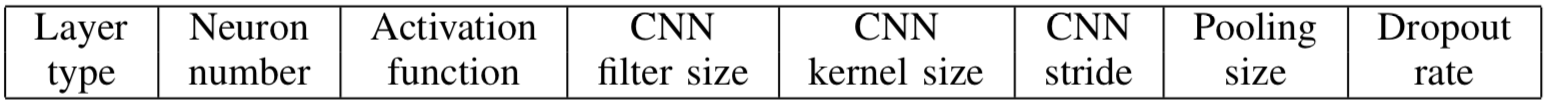
\includegraphics[width=0.48\textwidth]{img/array_layer.png}
\caption{Visual representation of a neural network layer as an array.}
\label{fig:neural_network_array}
\end{figure}

The proposed representations is capable of handling different types of neural network architectures, in principle this representation can handle multi-layer perceptrons (MLPs), convolutional neural networks (CNNs) and recurrent neural networks (RNNs). For any given neural network layer the array will only contain values for the entries that are applicable to the layer, values for other types of layers are set to 0.

\begin{comment}
\begin{table}[!htb]
\begin{center}
\scalebox{0.8}{
\begin{tabular}{| c | c | c | c | c | c | c | c |}
\hline
Layer & Number of & Activation & CNN & CNN & CNN & Pooling & Dropout\\
type & neurons & function & filter size & kernel size & stride & size & rate\\
\hline
\end{tabular}
}
\end{center}
\caption{Visual representation of a neural network layer as an array.}
\label{table:neural_network_array}
\end{table}
\end{comment}

Let us illustrate the proposed encoding with an example. The following example considers an MLP, thus only Layer type, Number of neurons, Activation function and Dropout rate entries are applicable, the rest will remain as 0. Consider $S_e$ as a model made up of several stacked layers as those shown in Figure \ref{fig:neural_network_array}.

\begin{align*}
S_e = \left[ \left[1, 264, 2, 0, 0, 0, 0, 0 \right], \left[5, 0, 0, 0, 0, 0, 0, 0.65 \right], \right. \\
\left. \left[1, 464, 2, 0, 0, 0, 0, 0 \right], \left[5, 0, 0, 0, 0, 0, 0, 0.35 \right], \right. \\
\left. \left[1, 872, 2, 0, 0, 0, 0, 0 \right], \left[1, 10, 3, 0, 0, 0, 0, 0 \right] \right]
\end{align*}


The neural network representation of the presented model is shown in Table \ref{table:neural_network_model}. \\

\begin{table}[!htb]
\begin{center}
\begin{tabular}{| c | c | c | c |}
\hline
Layer type & Neurons & Activation Function & Dropout Ratio \\
\hline
Fully connected & 264 & ReLU & n/a \\
Dropout & n/a & n/a & 0.65 \\
Fully Connected & 464 & ReLU & n/a\\
Dropout & n/a & n/a & 0.35\\
Fully Connected & 872 & ReLU & n/a\\
Fully Connected & 10 & Softmax & n/a\\
\hline
\end{tabular}
\end{center}
\caption{Neural network model.}
\label{table:neural_network_model}
\end{table}

Encoding the neural network as a list of arrays presents two big advantages over other representations. First, the number of layers that can be stacked is, in principle, arbitrary. Second, the validity of an architecture can be verified in constant time every time a new layer is to be stacked to the model, this is due to the fact that in order to stack a layer in between the model one just needs to check for compatibility between the previous and next layers. The ability of stacking layers dynamically and verifying its correctness as a new layer is stacked allows for a powerful representation that can build several kinds of neural networks such as fully connected, convolutional and recursive. The rules for stacking layers together are described in Table \ref{table:neural_network_building_rules}.

\subsection{Generating valid models}
\label{sec:valid_models}

Having the rules for stacking layers together, generating valid models is straightforward. An initial layer type has to be specified by the user, the initial layer type can be FullyConnected, Convolutional or Recurrent. Defining the initial layer type effectively defines the type of architectures that can be generated by the algorithm, i.e. if the user chooses FullyConected as the initial layer, all the generated models will be fully connected, if the user chooses Convolutional as initial layer the algorithm will generate Convolutional models only and so on.

Just as the initial layer type has to be user defined, the final/output layer is also user defined, in fact, all of the generated models share the same output layer. The output layer is always a FullyConnected layer, furthermore, it is generated based on the type of problem to solve (classification or regression). In the case of classification problems the number of neurons is defined by the number of classes in the problem and the softmax function is used as activation function. For regression problems the number of neurons is one and the activation function used is the linear function.

Having defined the architecture type and the output layer, generating an initial model is an iterative process of stacking new layers that comply with the rules in Table \ref{table:neural_network_building_rules}. A user defined parameter $n_p$ is used to stop inserting new layers, every time a new layer is stacked in the model a random number $n_r \in \left[0,1\right]$ is generated using the following probability distribution

\begin{equation}
n_r = 1 - \sqrt{1 - U},
\label{eq:more_layers_prob}
\end{equation}

where $U$ is a number drawn from a uniform distribution. If $n_r < n_p$ and if the current layer is compatible with the last layer (according to Table \ref{table:neural_network_building_rules}) then no more layers are inserted. Equation \ref{eq:more_layers_prob} is used to let the user choose the probability with which more layers are stacked to a neural network model, thus, if the user wants that a new layer is inserted with an $80\%$ of probability the user must choose $n_p = 0.8$. With regards to layers that have an activation function, even though in principle any valid combination is possible, for this application we choose to keep all the activations for similar layers the same across the model since this is usually the common practice. 

\subsection{Selection}
\label{sec:selection}

In order to generate $n_s$ offsprings $2n_s$ parents are required. The parents are chosen using a selection mechanism which takes the population $\mathcal{C}(t)$ at the current generation and returns a list of parents for crossover. For our application, the selection mechanism used is based on the binary tournament selection \cite{Engelbrecht2007, Krishnakumar1989}. A description of the mechanism is given next: 

\begin{itemize}
\item Select $m_s$ parents at random where $m_s < n_s$.
\item Compare the selected elements in a pair-wise manner and return the most fit individuals.
\item Repeat the procedure until $2n_s$ parents are selected.
\end{itemize}

It is important to note in the above procedure that the larger $m_s$ is, the more the probable that the best individual in the population is chosen as one of the parents, this is not a desirable behavior, thus we warn the users to keep $m_s$ small. Also, recall from Algorithm \ref{algorithm:nn_ea} that our approach uses elitism, therefore the best individual of a current generation remains unchanged in the next generation.

\subsection{Crossover operator}
\label{sec:crossover}

Since the encoding chosen for this task is rather peculiar the existing operators are not suitable for it, indeed, we designed a new crossover operator. In this section we describe in detail the proposed crossover operator. Our operator is based on the two point crossover operator for genetic algorithms \cite{holland1992} in the sense that two points are selected for each parent, nevertheless our operator is more restrictive, as to which pairs of points may be selected, in order to ensure the generation of valid architectures. 

The key concept behind our crossover operator is that of  ``compatibility between pairs of points''. Consider two models $S_1, S_2$ that will serve as parents for one offspring, assume that the offspring will be generated by replacing some layers in $S_1$ from some layers in $S_2$, $S_1$ is thus the base parent. If we selected any two pairs of points $(r_1, r_2)$ from $S_1$ and $(r_3, r_4)$ from $S_4$ it may happen that such pairs of points can not be interchangeable (because layer $r_3$ can not be placed instead of layer $r_1$ or layer $r_4$ can not be placed instead of layer $r_2$). Therefore, the selection mechanism must ensure that the interchange points, $(r_1, r_2), (r_3, r_4)$, are compatible, i.e. that is that layer $r_3$ is compatible with the layer preceding $r_1$ and that the layer after $r_2$ is compatible with layer $r_4$, compatibility is defined in terms of the rules described in Table \ref{table:neural_network_building_rules}. A selection mechanism that guarantees this compatibility between pairs of points is described in Algorithm \ref{algorithm:crossover_method}, as mentioned before, this method assumed that the offspring will be generated by replacing some layers in $S_1$ from some layers in $S_2$ .

\begin{algorithm}[!htb]
\caption{Crossover Method}
\begin{algorithmic}
%\Procedure{Basic Evolutionary Algorithm}{$a,b$}\Comment{The g.c.d. of a and b}
\State Let $S_1, S_2$ be the arrays containing the stacked layers of a neural network model in parents 1 and 2 respectively.
\State Take two random points $(r_1, r_2)$ from $S_1$ where $r_1 <= r_2 $
\If{$r_1 = r_2 $} 
	\State {$r_2 = len(S_1-1)$} 
\Else 
	\State{pass} 
\EndIf
\State Find all the pairs of points $(r_3, r_4)_i$ in $S_2$ that are compatible with $(r_1, r_2)$ where $r_3 < r_4$ and $(r_4 - r_3) - (r_2 - r_1) < \mathcal{L}$
\State Randomly pick any of the pairs $(r_3, r_4)_i$
\State Replace the layers in $S_1$ between $r_1, r_2$ inclusive with the layers in $S_2$ between $r_3, r_4$ inclusive. Label the new model as $S_3$
\State Rectify the activation functions of $S_3$ to match the activation functions of $S_1$
\end{algorithmic}
\label{algorithm:crossover_method}
\end{algorithm}

It is possible that the mechanism described Algorithm \ref{algorithm:crossover_method} requires more than one attempt to find valid interchange points, $(r_1, r_2), (r_3, r_4)$, for models $S_1$ and $S_2$. Based on our experience with the method and the obtained results,  Algorithm \ref{algorithm:crossover_method} usually requires only one attempt to successfully generate a valid offspring, nevertheless to prevent the crossover mechanism from getting trapped in an infinite loop we limit the number of trials done to $n_c$, where $n_c=3$ is the default but can be adjusted by the user to its needs. Let us illustrate Algorithm \ref{algorithm:crossover_method} with an example. Consider the following models:

\begin{align*}
S_1 & = \left[ \left[1, 264, 2, 0, 0, 0, 0, 0 \right], \left[5, 0, 0, 0, 0, 0, 0, 0.65 \right], \right. \\
& \left. \left[1, 464, 2, 0, 0, 0, 0, 0 \right], \left[5, 0, 0, 0, 0, 0, 0, 0.35 \right], \right. \\
& \left. \left[1, 872, 2, 0, 0, 0, 0, 0 \right], \left[1, 10, 3, 0, 0, 0, 0, 0 \right] \right]
\end{align*}

\begin{align*}
S_2 & = \left[ \left[1, 56, 0, 0, 0, 0, 0, 0 \right], \left[5, 0, 0, 0, 0, 0, 0, 0.25 \right], \right. \\
&  \left. \left[1, 360, 0, 0, 0, 0, 0, 0 \right], \left[1, 480, 0, 0, 0, 0, 0, 0 \right] \right. \\
&  \left. \left[1, 88, 0, 0, 0, 0, 0, 0 \right], \left[5, 0, 0, 0, 0, 0, 0, 0.2 \right], \right. \\
&  \left. \left[1, 10, 3, 0, 0, 0, 0, 0 \right] \right]
\end{align*}

Lets take $r_1 = 1$ and $r_2 = 3$, since these points are going to be removed from the model we need to find the compatible layers with $S_1[r_1-1]$ and $S_1[r_2]$ according to the rules described in Table \ref{table:neural_network_building_rules}. Note however that if $r_1 = 0$, i.e. the initial layer, then only a layer whose layer type is equal to the layer type of $S_1[0]$ is compatible. Thus, for this example the compatible pairs of points $(r_3, r_4)_i$ are:

\begin{align*}
& \left[ (0, 0), (0, 2), (0, 4), (0, 5), (1, 2), (1, 4), (1, 5), \right. \\
& \left. (2, 2), (2, 4), (2, 5), (4, 4), (4, 5), (5, 5) \right]
\end{align*} 

Assume we pick at random the pair $(2,4)$, thus the offspring, which we will call $S_3$, looks like:

\begin{align*}
S_3 & = \left[ \left[1, 264, 2, 0, 0, 0, 0, 0 \right], \left[1, 360, 2, 0, 0, 0, 0, 0 \right], \right. \\
& \left. \left[1, 480, 2, 0, 0, 0, 0, 0 \right] , \left[1, 88, 2, 0, 0, 0, 0, 0 \right], \right. \\
& \left. \left[1, 872, 2, 0, 0, 0, 0, 0 \right], \left[1, 10, 3, 0, 0, 0, 0, 0 \right] \right]
\end{align*}

which is a valid model. The reader is encouraged to check the actual neural network representations for each of the models in this example in Tables \ref{table:neural_network_model_S1} to \ref{table:neural_network_model_S3}. Notice though that all the activation functions of the same layer types are changed to match the activation functions of the first parent $S_1$. We call this process ``activation function rectification'' and it basically implies changing all the activation functions of the layers that share the same layer type between $S_1$ and $S_3$ to the activation functions used in $S_1$. 

Finally, one important feature of this crossover operator is that it has the ability to generate neural network models of different sizes, i.e. it can shrink or increase the size of the base parent. This behavior mimics that of machine learning practitioners, which will often start with a base model and iteratively shrink or increase the size of the base model in order to find the one that has the best inference performance.

\subsection{Mutation operator}
\label{sec:mutation}

The mutation operator is used to induce small changes to some of the models generated through the crossover mechanism. In the realm of evolutionary computation these subtle changes tend to improve the exploration properties of the current population (genetic diversity) by injecting random noise to the current solutions.  Although according to \cite{Krishnakumar1989} mutation is not needed in the micro-GA, we believe some sort of mutation is needed in our application in order to get more diverse models which could potentially lead to better inference abilities, nevertheless, our mutation approach will be less disruptive in order to mitigate its effect. Following the same ideas found on the literature we developed a mutation operator to handle neural network models.

As stated above our mutation approach is less disruptive than the common mutation operators \cite{Engelbrecht2007}, this decision follows two main reasons: First, is the fact that usually micro genetic algorithms don't make use of the mutation algorithm since the crossover operator has already induce significant genetic diversity in the population. The second reason is related to the way neural networks are usually built by human experts, commonly experts try a number of models and then make subtle changes to each of them in order to try to improve the inference ability of them, such changes usually involve changing the parameters in a layer, adding or removing a layer, adding regularization or changing the activation functions. 

Based on the principles described above, our mutation process randomly chooses one layer, using a probability $m_p$, of the model and then proceeds to make one of the following operations:

\begin{itemize}
\item Change a parameter of the layer chosen for a value complying the values stated in Table \ref{table:neural_network_array_details}.
\item Change the activation function of the layer. This would involve rectifying the entire model (described in section \ref{sec:crossover}).
\item Add a dropout layer if the chosen layer is compatible.\\
\end{itemize} 

This operations together provide a rich set of possibilities for performing efficient mutation while still keeping valid models after mutation is performed. 

\subsection{Determining nominal convergence}
\label{sec:convergence}

Nominal convergence is one of the criteria used for early stopping of the evolutionary procedure of our algorithm. Some literature defines the convergence in terms of the fitness of the individuals \cite{Engelbrecht2007}, while in \cite{Krishnakumar1989} the convergence is defined in terms of the genotype or phenotype of the individuals. Although convergence based on the actual fitness of the individuals may be easier to asses given that the fitness is already calculated, we believe that an assessment of convergence based on the actual genotype of the individuals suits our needs better, this follows the following reasoning.

Since neural networks are stochastic in nature, we expect some variations in the fitness of the individuals at every different run, furthermore since we are running the training process for only few epochs (in order to avoid a high computational burden) the performance of the networks can be quite different and would not be a reliable indicator of convergence. Instead, to assess convergence we look at the genotype and compute the similarities between the different individuals.

To compute the similarities between different individuals we take the following approach. Let $S_1, S_2$ where $len(S_2) >= len(S_1)$ be the genotype representing two different models, let also $S_1 - S_2$ represent the layer-wise difference between each model and $S_i[j]$ be the array representation of the $j-th$ layer of model $i$, $S_2 - S_1$ is defined in Algorithm \ref{algorithm:difference_between_networks}. \\

\begin{algorithm}[!htb]
\caption{$S_2 - S_1$ Method}
\begin{algorithmic}[0]
%\Procedure{Basic Evolutionary Algorithm}{$a,b$}\Comment{The g.c.d. of a and b}
\State Let $d \in \mathbb{R}$ be the distance between the two models. Make $d = 0$
\For{Each layer $i$ in $S_1$ except last layer}
	\State{$d = d + norm_2(S_2[i]-S_1[i])$}
\EndFor
\For{Each remaining layer $i$ in $S_2$ except last layer}
	\State{$d = d + norm_2(S_2[i])$}
\EndFor
\State Return $d$
\end{algorithmic}
\label{algorithm:difference_between_networks}
\end{algorithm}

This method is computationally inexpensive since the size of the population is small. Furthermore, it helps accurately establish the similarity between any two neural networks, given two neural network models $S_1$ and $S_2$ is $S_1 = S_2$ then $S_2 - S_1 = 0$. For our purposes we stop the algorithm and launch the new experiment if the distance between any $s$ models is smaller than $c$ where both $s$ and $c$ are user defined parameters.

\subsection{Implementation}
\label{sec:implementation}

AutoNN is implemented in about 700 lines of code in Python. The code can be found in \url{https://github.com/dlaredo/automatic_model_selection}. We took a functional programming approach for its implementation. The models $S_i$ generated by the algorithm are fetched to Keras \cite{keras2015} and then evaluated, nevertheless the models can be evaluated in any other framework such as TensorFlow or Pytorch and even using different programming languages such as C++ for performance reasons.

In order to boost performance we make use of Ray \cite{Moritz2017} which is a distributed computing framework tailored for AI applications. In order to distribute workloads in Ray developers only have to define Remote Functions make use of Python annotations, Ray will then distribute these Remote Functions across the different nodes in the cluster. There are three different types of nodes in Ray: Drivers, Workers and Actors. A Driver is the process executing the user program, a Worker is a stateless process that executes remote functions invoked by a driver or another worker, finally, an Actor is a statefull process that executes, when invoked, the methods it exposes.

For our implementation we code the individual fetching to Keras and its fitness evaluation as Ray Remote Functions (Workers), while the rest of our algorithm is implemented within the Driver, therefore the partial train of each neural network within the current population is performed in a distributed way, highly increasing the performance of our algorithm. Furthermore since the only messages being sent over the cluster are arrays (the neural network representation $S_i$) and the fitness of the neural network model $f$ there is little chance that the data interchanged causes a bottleneck or increases latency in the system.

\section{Evaluation}
\label{sec:evaluation}

We evaluate AutoNN with two different datasets, each of which is a different type of inference problem. Our results are compared against baseline implementations and state-of-the-art methods for automatic model selection. In particular we compare our results against AutoWeka \cite{Thornton2016}, PyBrain \cite{Schaul2010} and MLLib \cite{mlib2017}.

For the experiments in this section each model generated by AMS was trained using the following parameters:

\begin{table}[!htb]
\begin{center}
\scalebox{0.85}{
\begin{tabular}{| c | c | c | c | c | c |}
\hline
Dataset & Epochs & Learning Rate & Optimizer & Loss function & Metrics \\
\hline
\multirow{2}{*}{MNIST} & \multirow{2}{*}{5} & \multirow{2}{*}{0.001} & \multirow{2}{*}{Adam} & Categorical & Categorical\\
		  &     &		   &			 & crossenthropy & 	accuracy\\
CMAPSS & 5 & 0.01 & Adam & MSE & MSE\\
\multirow{2}{*}{CIFAR10} & \multirow{2}{*}{5} & \multirow{2}{*}{0.001} & \multirow{2}{*}{Adam} & Categorical & Categorical\\
		  &     &		   &			 & crossenthropy & 	accuracy\\
\hline
\end{tabular}
}
\end{center}
\caption{Training parameters for each of the used datasets.}
\label{table:training_params}
\end{table}

For CMAPSS dataset we used a larger learning rate since we are evaluating the model using very few epochs for this complex problem, therefore, in order to get a clearer idea of which individuals within the population may be promising we speed up the training process by increasing the learning rate.

\subsection{MNIST Dataset - A classification problem}

We first test our algorithm on the MNIST Dataset \cite{Lecun2010}. The MNIST Dataset of handwritten digits is one of the most commonly used datasets for evaluating the performance of neural networks. It has a training set of 60,000 examples and a test set of 10,000 examples. The digits have been size-normalized and centered in a fixed-size image, the size of each image is of 28x28 pixels. Ass part of the data pre-processing step we normalized all the pixels in each image to be in the range of $[0,1]$ and unrolled the 28x28 image into a vector with 784 components.

We use MNIST dataset as a baseline for measuring the performance of our approach, furthermore, we use MNIST to analyze each one of the major components of AutoNN. Given the popularity of MNIST, several neural networks with varying degrees of accuracy have been proposed, therefore it is easy to find good models to compare with. 

We start by running AutoNN to find a suitable FullyConnected model for classification for the MNIST dataset. The details for the parameters used in this test are described in Table \ref{table:MNIST_params}

\begin{table}[!htb]
\begin{center}
\begin{tabular}{| c | c |}
\hline
Parameter & AutoNN Value \\
\hline
Problem Type & 1 \\
Architecture Type & FullyConnected \\
Input Shape & $(784, M)$  \\
Output Shape & $(10, M)$ \\
Cross Validation Ratio & $c_v = 0.2$ \\
Mutation Ratio & $m_p = 0.4$ \\
More Layers Probability & $n_r = 0.7$ \\
Network Size Scaling Factor & $\alpha = 0.8$ \\
Population Size & $n_s = 10$ \\
Tournament Size & $n_t = 4$ \\
Max Similar Models & $s = 3$ \\
Total Experiments & $E_{max} = 5$ \\
\hline
\end{tabular}
\end{center}
\caption{Parameters for MNIST for each method.}
\label{table:MNIST_params}
\end{table}

We first take a look at the generated initial population. For the sake of space we will only discuss the sizes of the models, furthermore we will make a small change in our notation for describing neural network models, for the remainder of this section we denote a layer of a neural network as $(n_e, a_f)$ where $n_e$ denotes the number of neurons in case the layer is fully connected or the dropout rate in case the layer is a dropout layer and $a_f$ denotes the activation function of the later if the layer is a fully connected layer. The initial five generated individuals are presented next. Fitness, accuracy and raw size of the models in the initial population are presented in Table \ref{table:autonn_mnist_initial}

\begin{align*}
S_1 & = \left[ (280, 1), (32, 1), (0.4), (304, 1), (96, 1), \right.\\
& \left. (0.55), (600, 1), (10, 3) \right] \\
S_2 & = \left[ (96, 0), (0.55), (168, 0), (10, 3) \right] \\
S_3 & = \left[ (1024, 2), (560, 2), (0.15), (360, 2), (624, 2), \right.\\
& \left. (0.5), (144, 2), (616, 2), (504, 2), (776, 2), (0.3), \right.\\ 
& \left. (8, 2), (200, 2), (0.2), (904, 2), (0.35), (664, 2), \right.\\ 
& \left. (0.35), (904, 2), (0.65), (488, 2), (0.4), (448, 2), \right.\\
& \left. (216, 2), (336, 2), (368, 2), (400, 2), (0.2), \right.\\
& \left. (112, 2), (48, 2), (0.3), (944, 2), (584, 2), (128, 2), \right.\\
& \left. (0.15), (376, 2), (288, 2), (816, 2), (10, 3) \right] \\
S_4 & = \left[ (672, 0), (840, 0), (0.25), (384, 0), (400, 0), \right.\\
& \left. (712, 0), (10, 3) \right] \\
S_5 & = \left[ (472, 1), (968, 1), (0.4), (816, 1), (104, 1), \right.\\
& \left. (0.5), (488, 1), (192, 1), (0.4), (256, 1), (10, 3) \right] \\
\end{align*}

\begin{comment}
\begin{align*}
S_1 & = \left[ (968, 0), (688, 0), (10, 3) \right] \\
S_2 & = \left[ (824, 2), (0.4), (168, 2), (808, 2), (528, 2), (10, 3) \right] \\
S_3 & = \left[ (136, 1), (984, 1), (144, 1), (680, 1), (10, 3) \right] \\
S_4 & = \left[ (712, 2), (0.3), (96, 2), (368, 2), (584, 2), (240, 2) \right. \\
& \left. (256, 2), (0.65), (384, 2), (536, 2), (648, 2), (0.3), (88, 2), (10, 3) \right] \\
S_5 & = \left[ (448, 0), (0.3), (888, 0), (10, 3) \right] \\
\end{align*}
\end{comment}

\begin{table}[!htb]
\begin{center}
\begin{tabular}{| c | c | c | c |}
\hline
Model & Score (Accuracy) & Trainable Parameters & Fitness\\
\hline
$S_1$ & 94.6\% & 332314 & 4.9519\\
$S_2$ & 91.5\% & 93346 & 4.1827\\
$S_3$ & 10.5\% & 6305682 & 14.3839\\
$S_4$ & 92.0\% & 1862426 & 5.8084\\
$S_5$ & 95.0\% & 1901162 & 5.5140\\
\hline
\end{tabular}
\end{center}
\caption{Scores for the initial population found by AutoNN for MNIST. $\alpha = 0.8$}
\label{table:autonn_mnist_initial}
\end{table} 

First thing we can observe is that the sizes of the models are widely variable, with some models having as few as 1 hidden layer and some having more than 20 hidden layers, another thing to note is the variability in terms of activation functions with some models using sigmoid, some using tanh and some using relu as activation functions.

The next thing to notice is the fitness of each of the initial individuals with the worst individual in the population ($S_3$) being extremely unfit due to the large size of the network (more than 6 million trainable parameters) and the low accuracy of the model (about $10\%$). The rest of the individuals display a decent accuracy (about $90\%$ of accuracy) but they exhibit a large number of trainable parameters. Since MNIST is a simple dataset to infer for modern neural networks it is observable that most of the neural networks at the initial population already attain acceptable accuracy, nevertheless in this specific case, the size of the network can be greatly improved. In the next sections we will show how AMS optimizes the accuracy along with the size of the models for more complex datasets.

For this test, after the 10 generations, the algorithm converged to $S^*_1 = \left[ (96, 1), (10, 3) \right]$, where * denotes the best individual in the population and the subindex denotes the experiment number.

We now run the same experiment four more times for a total of five different experiments with the same parameter settings for AMS. The obtained models are presented next, the fitness, accuracy and raw size of the models are presented in Table \ref{table:autonn_mnist_1}. The best overall model is $S^* = S^*_2$.

\begin{align*}
S^*_1 & = \left[ (96, 1), (10, 3) \right] \\
S^*_2 & = \left[ (48, 2), (48, 2), (10, 3) \right] \\
S^*_3 & = \left[ (408, 2), (10, 3) \right] \\
S^*_4 & = \left[ (296, 1),  (10, 3) \right] \\
S^*_5 & = \left[ (128, 1), (128, 1), (0.3),  (10, 3) \right] \\
\end{align*}

\begin{table}[!htb]
\begin{center}
\begin{tabular}{| c | c | c | c |}
\hline
Model & Score (Accuracy) & Trainable Parameters & Fitness\\
\hline
$S^*_1$ & 94.4\% & 76330 & 4.4638\\
$S^*_2$ & 95.0\% & 40522 & 4.1827\\
$S^*_3$ & 96.8\% & 224370 & 4.7226\\
$S^*_4$ & 95.1\% & 235330 & 4.7843\\
$S^*_5$ & 95.5\% & 118282 & 4.5016\\
\hline
\end{tabular}
\end{center}
\caption{Scores for the best models found by AutoNN for MNIST. $\alpha = 0.8$}
\label{table:autonn_mnist_1}
\end{table}

As can be observed in Table \ref{table:autonn_mnist_1} small models are preferred, furthermore there seems to be a preference for tanh activation functions. The fact that small models are preferred over larger models, despite the fact that larger models may yield better performance, is due to the value of the weighting factor $\alpha = 0.8$ which highly penalizes the overall size (number of trainable parameters) of the neural network.  Let us further illustrate this behavior by running the algorithm with $\alpha = 1$ and $\alpha = 0.6$.

The best models for each experiment with $\alpha = 0.6$, are listed next, the fitness and raw size of the models are described in Table \ref{table:autonn_mnist_2}. The best overall model is $S^* = S^*_5$.

\begin{align*}
S^*_1 & = \left[ (312, 2), (10, 3) \right] \\
S^*_2 & = \left[ (368, 2), (0.15), (10, 3) \right] \\
S^*_3 & = \left[ (200, 1), (10, 3) \right] \\
S^*_4 & = \left[ (224, 2),  (10, 3) \right] \\
S^*_5 & = \left[ (88, 2), (88, 2), (10, 3) \right] \\
\end{align*}

\begin{table}[!htb]
\begin{center}
\begin{tabular}{| c | c | c | c |}
\hline
Model & Score (Accuracy) & Trainable Parameters & Fitness\\
\hline
$S^*_1$ & 96.7\% & 248050 & 3.5575\\
$S^*_2$ & 96.8\% & 292570 & 3.5976\\
$S^*_3$ & 96.3\% & 159010 & 3.4891\\
$S^*_4$ & 96.3\% & 178090 & 3.5169\\
$S^*_5$ & 95.2\% & 77802 & 3.4094\\
\hline
\end{tabular}
\end{center}
\caption{Scores for the best models found by AutoNN for MNIST, $\alpha = 0.6$.}
\label{table:autonn_mnist_2}
\end{table}

The results in Table \ref{table:autonn_mnist_2} display larger models with respect to those displayed in Table \ref{table:autonn_mnist_1}. This is due to the relaxation on the $\alpha$ parameter which takes more into account the accuracy of the model rather than the size of the network itself. Nevertheless, it can be observed that the accuracy of the obtained models when $\alpha=0.6$ is just slightly better than the results obtained with $\alpha=0.8$, this is likely due to the fact that MNIST dataset is usually easy to classify using neural networks. We will further analyze this behavior using other datasets in the next sections.

Next we repeat the experiment with $\alpha = 1$, again the obtained models are listed next and their fitness and raw size of the models are described in Table \ref{table:autonn_mnist_3}. The best overall model is $S^* = S^*_2$.

\begin{align*}
S^*_1 & = \left[ (136, 2), (136, 2), (0.35), (10, 3) \right] \\
S^*_2 & = \left[ (32, 1), (32, 1), (10, 3) \right] \\
S^*_3 & = \left[ (56, 2), (0.1), (10, 3) \right] \\
S^*_4 & = \left[ (152, 1), (152, 1), (10, 3) \right] \\
S^*_5 & = \left[ (64, 2),  (10, 3) \right] \\
\end{align*}

\begin{table}[!htb]
\begin{center}
\begin{tabular}{| c | c | c | c |}
\hline
Model & Score (Accuracy) & Trainable Parameters & Fitness\\
\hline
$S^*_1$ & 96.5\% & 126762 & 5.4529\\
$S^*_2$ & 93.9\% & 26506 & 5.0388\\
$S^*_3$ & 94.1\% & 44530 & 5.2348\\
$S^*_4$ & 96.0\% & 144106 & 5.5550\\
$S^*_5$ & 94.6\% & 50890 & 5.2475\\
\hline
\end{tabular}
\end{center}
\caption{Scores for the best models found by AutoNN for MNIST, $\alpha = 1$.}
\label{table:autonn_mnist_3}
\end{table}


The results in Table \ref{table:autonn_mnist_3} show that when the number of trainable parameters has a large impact on the overall fitness of the individuals, the algorithm tends to prefer smaller networks, this is specially useful for cases where the computational power is limited, such as embedded systems. This brings an obvious drawback, namely that neural networks that exhibit a lower performance as compared to larger neural networks may be preferred. Nevertheless, this tradeoff can be controlled by the user by varying the $\alpha$ parameter. 

Note that the change in fitness among the three experiments is due to the fact that the size of the neural network was scaled (See equation \ref{eq:fitness_function_scaled}) and thus there is no fair way of comparing the fitness of the models shown Tables \ref{table:autonn_mnist_1}, \ref{table:autonn_mnist_2} and \ref{table:autonn_mnist_3} against each other.

Finally, we compare the best models for each value of $\alpha$ against each other. A 10-fold cross-validation process, with a training of 50 epochs per fold, was carried out for each one of the best models in order to obtain the mean accuracy for each model. We denote $ S^*_1$ as the best model corresponding to $\alpha = 0.6$, $S^*_2$ is the model corresponding to $\alpha = 0.8$ and $S^*_3$ is the model corresponding to $\alpha = 1$. We also measure the accuracy of each of the models using a test set that was never used during the training or tuning processes of the models. The accuracy averages and size of the networks are summarized in Table \ref{table:avg_accuracies_mnist}. The experiments for each $\alpha$ value took about 8.5 minutes in our test rig.

\begin{table}[!htb]
\begin{center}
\begin{tabular}{| c | c | c | c |}
\hline
Model & 10-fold Avg. Score & Test Avg. Score & Network size\\
\hline
$S^*_1$ & 97.6\% & 97.7\% & 93346\\
$S^*_2$ & 97.0\% & 97.2\% & 77802\\
$S^*_3$ & 96.1\% & 96.4\% & 26506\\
\hline
\end{tabular}
\end{center}
\caption{Accuracy obtained by each of the top 3 models for MNIST dataset.}
\label{table:avg_accuracies_mnist}
\end{table}

As expected, model $S^*_3$ yields a smaller neural network (about 3 times smaller) than the rest of the proposed models, nevertheless its accuracy is the worst of the three models (though by a small margin). On the contrary model $S^*_1$ gets the best performance (again marginal) in terms of accuracy but with a larger neural network as compared to model $S^*_3$. Finally, model $S^*_2$ as expected, attains a performance in between $S^*_1$ and $S^*_3$ with a number of trainable parameters also in between $S^*_1$ and $S^*_3$. It is important to note though that the accuracy of each of the models presented for this dataset is acceptable as compared against some modern methods. Table \ref{table:MNIST_results_top} shows the top models along with their obtained accuracy for the MNIST dataset, it can be observed that the accuracy obtained by AMS is close to that obtained by fine tuned models. A thorough comparison between the obtained models and some other modern models using this dataset is out of the scope of this work mainly fue to the fact that the models obtained by AMS are not fine tuned as the models with higher accuracy.

\begin{table}[!htb]
\begin{center}
\begin{tabular}{| c | c | c |}
\hline
Method & Test accuracy & Size\\
\hline
3 Layer NN, 300+100 hidden units \cite{lecun-98} &  96.95\% & 266610\\
2 Layer NN, 800 hidden units \cite{Simard2003} & 98.4\% & 636010\\
6-layer NN (elastic distortions) \cite{Ciresan2010}  & 99.65\% & 11972510\\
\hline
\end{tabular}
\end{center}
\caption{Top results for MNIST dataset.}
\label{table:MNIST_results_top}
\end{table}

Comparing the models obtained by AMS agains the models in Table \ref{table:MNIST_results_top} we can observe that eventhough AMS models don't attain the highest accuracy they exhibit good inference capabilities with a much lesser number of trainable parameters (size of the model). This shows that AMS models show a good balance between the inference power of the model and its overall size, furthermore the score-size tradeoff can be controlled by means of the $\alpha$ parameter, where a value closer to $\alpha=0$ makes AMS prefer networks with higher scores and a value closer to $\alpha = 1$ makes AMS prefer networks with smaller sizes.


\subsection{CMAPSS Dataset - A regression problem}

In this section we analyze the performance of AMS when working with regression problems. For testing regression we use the C-MAPSS dataset \cite{CMAPS2008}. The C-MAPSS dataset contains simulated data produced using a model based simulation program developed by NASA. The dataset is further divided into 4 subsets composed of multi-variate temporal data obtained from 21 sensors, nevertheless for our test we will only make use of the first subset of data. Training and separate test sets are provided. The training set includes run-to-failure sensor records of multiple aero-engines collected under different operational conditions and fault modes.

The data is arranged in an $n\times26$ matrix where $n$ is the number of data points in each subset. The first two variables represent the engine and cycle
numbers, respectively. The following three variables are operational settings which correspond to the conditions in Table \ref{table:dataset_cmaps_params} and have a
substantial effect on the engine performance. The remaining variables represent the 21 sensor readings that contain the information about the engine
degradation over time.

\begin{table}[!htb]
\begin{center}
\scalebox{0.90}{
\begin{tabular}{| c | c | c | c |}
\hline
Train trajectories & Test trajectories & Operating conditions & Fault modes \\
\hline
100 & 100 & 1 & 1 \\
\hline
\end{tabular}
}
\end{center}
\caption{CMAPSS dataset details.}
\label{table:dataset_cmaps_params}
\end{table}

Each trajectory within the training and test sets represents the life cycles of the engine. Each engine is simulated with different initial health conditions, i.e. no initial faults. For each trajectory of an engine the last data entry corresponds to the cycle at which the engine is found faulty. On the other hand, the trajectories of the test sets terminate at some point prior to failure, hence the need to predict the remaining useful life (RUL). The aim of the MLP model is to predict the RUL of each engine in the test set via regression. The actual RUL values of test trajectories are also included in the dataset for verification. Further discussions of the dataset and details on how the data is generated can be found in \cite{Saxena2008}.

For this test we follow the data pre-processing described in \cite{Laredo2018}, in short only 14 out of the total 21 sensors are used as the input data. Furthermore we also use a strided time-window, with window size of 24, a stride of 1 and earlyRUL of 129, to form the feature vectors for the MLP as in \cite{Laredo2018}. Further details of the time-window approach can be found in \cite{Laredo2018} and \cite{Li2018}.

We run AMS to find a suitable FullyConnected model for regression using the CMAPSS dataset. The details for the parameter used in this test are described in Table \ref{table:CMAPSS_params}

\begin{table}[!htb]
\begin{center}
\begin{tabular}{| c | c |}
\hline
Parameter & AutoNN Value \\
\hline
Problem Type & 1 \\
Architecture Type & FullyConnected \\
Input Shape & $(336, M)$  \\
Output Shape & $(1, M)$ \\
Cross Validation Ratio & $c_v = 0.2$ \\
Mutation Ratio & $m_p = 0.4$ \\
More Layers Probability & $n_r = 0.7$ \\
Network Size Scaling Factor & $\alpha = 0.8$ \\
Population Size & $n_s = 10$ \\
Tournament Size & $n_t = 4$ \\
Max Similar Models & $s = 3$ \\
Total Experiments & $E_{max} = 5$ \\
\hline
\end{tabular}
\end{center}
\caption{Parameters for CMAPSS for each method.}
\label{table:CMAPSS_params}
\end{table}

Once again we start by presenting the baseline for our tests. Table \ref{table:CMAPSS_results_top} presents some of the top results obtained by MLPs in the CMAPSS dataset, the results are measured in terms of the RMSE (Root Mean Squared Error) between the real RUL and the predicted RUL. 

\begin{table}[!htb]
\begin{center}
\begin{tabular}{| c | c | c |}
\hline
Method & Test RMSE & Network size \\
\hline
Time Window MLP \cite{Lim2016} & 15.16 & 6041\\
Time Window MLP with EA \cite{Laredo2018} & 14.39 & 7161\\
Deep MLP ensemble \cite{Zhang2016} & 15.04 &  n/a \\
\hline
\end{tabular}
\end{center}
\caption{Top results for CMAPSS dataset.}
\label{table:CMAPSS_results_top}
\end{table}

As with MNIST dataset we performed experiments for $\alpha \in \{0.6, 0.8, 1\}$. The best global models (best out of the five experiments) obtained for each of the $\alpha$ values are shown in Table \ref{table:avg_rmse_cmapss} along with their scores for CMAPSS data (RMSE) and the sizes of the networks. $S^*_1$ denotes the best model for $\alpha = 0.6$, while $S^*_2$ and $S^*_3$ denote the best models for $\alpha = 0.8$ and $\alpha = 1$ respectively. The experiments for each $\alpha$ value took about 3.5 minutes in our test rig.

\begin{table}[!htb]
\begin{center}
\begin{tabular}{| c | c | c | c |}
\hline
Model & 10-fold Avg. Score & Test Avg. Score & Network size\\
\hline
$S^*_1$ & 15.16 & 16.12 & 57809\\
$S^*_2$ & 15.20 & 14.83 & 9177\\
$S^*_3$ & 15.00 & 14.96 & 6817\\
\hline
\end{tabular}
\end{center}
\caption{RMSE obtained by each of the top 3 models for CMAPSS dataset.}
\label{table:avg_rmse_cmapss}
\end{table}

The results presented in Table \ref{table:avg_rmse_cmapss} further demonstrate the impact of the $\alpha$ parameter. As can be observed the size of the networks grow as $\alpha$ is relaxed (smaller). It can also be observed that the results obtained by the three proposed models in the Cross-Validation sets are very close among each other, nevertheless it is important to point out that $S^*_1$ attained such score with a larger network as compared with $S^*_2$ and $S^*_3$ whose sizes are fairly similar. This is mainly because the CMAPSS dataset does not require very large neural networks, therefore small models are usually preferred. 

The obtained models are also competitive when compared against some of the latest MLPs used with CMAPSS dataset (\ref{table:CMAPSS_results_top}). In this case we compare against the score obtained in the test set for each of the models. It is shown that two of the three models obtained by AMS obtain a better score than two (Time Window MLP and Deep MLP ensemble) of the three compared models, furthermore, the sizes of the proposed networks are as small as the sizes of the compared models. 



\section{Conclusions and Future Work}
\label{sec:conclusions}

In this paper we presented AutoNN, a new evolutionary algorithm for efficiently finding suitable neural network models for both classification and regression problems. Making use of efficient mutation and crossover operators the AutoNN is able to generate valid and efficient neural networks, in terms of both the size of the network and its performance. Furthermore, AutoNN is intrinsically distributable, exploiting this feature with the use of Ray \cite{Moritz2017} we were able to find efficient models for the MNIST dataset \cite{Lecun2010}.

Future work will consider more complex neural network architecturs such as LSTM and CNNs, techniques for assembling entire neural network pipelines will also be explored in future as well as the inclusion of more hyperparameters in the tuning process. Finally a better way of measuring distance between two neural network architectures will be explored, since this last element is of high importance for applications such as visualization and evolutionary computation.


\begin{comment}
Our proposal includes the comparisson of an evolutionary algorithm against sequential model based optimization for the selection of an optimal model, along with sampling and pruning techniques to only keep the most promising models and discard the rest of them. Furthermore, we propose to train multiple models simultaneously using Ray and perform bandit allocation resource to perform efficient resource allocation towards the most promising models. Our results will be fisrt tested using the CMAPSS dataset \cite{CMAPS2008} for regression and the MNIST dataset \cite{Lecun2010} for classification. A comparisson against AutoWEKA and Auto-sklearn (on the neural networks) will also be provided.
\end{comment}


% if have a single appendix:
%\appendix[Proof of the Zonklar Equations]
% or
%\appendix  % for no appendix heading
% do not use \section anymore after \appendix, only \section*
% is possibly needed

% use appendices with more than one appendix
% then use \section to start each appendix
% you must declare a \section before using any
% \subsection or using \label (\appendices by itself
% starts a section numbered zero.)
%

\begin{comment}
\appendices
\section{Proof of the First Zonklar Equation}
Appendix one text goes here.

% you can choose not to have a title for an appendix
% if you want by leaving the argument blank
\section{}
Appendix two text goes here.


% use section* for acknowledgment
\section*{Acknowledgment}


The authors would like to thank...


% Can use something like this to put references on a page
% by themselves when using endfloat and the captionsoff option.
\ifCLASSOPTIONcaptionsoff
  \newpage
\fi

\end{comment}



% trigger a \newpage just before the given reference
% number - used to balance the columns on the last page
% adjust value as needed - may need to be readjusted if
% the document is modified later
%\IEEEtriggeratref{8}
% The "triggered" command can be changed if desired:
%\IEEEtriggercmd{\enlargethispage{-5in}}

% references section

% can use a bibliography generated by BibTeX as a .bbl file
% BibTeX documentation can be easily obtained at:
% http://mirror.ctan.org/biblio/bibtex/contrib/doc/
% The IEEEtran BibTeX style support page is at:
% http://www.michaelshell.org/tex/ieeetran/bibtex/
%\bibliographystyle{IEEEtran}
% argument is your BibTeX string definitions and bibliography database(s)
%\bibliography{IEEEabrv,../bib/paper}
%
% <OR> manually copy in the resultant .bbl file
% set second argument of \begin to the number of references
% (used to reserve space for the reference number labels box)

\bibliographystyle{unsrt}
\bibliography{reference_model_selection}


\clearpage


\onecolumn%
\begin{table}[!htb]
\begin{center}
\begin{tabular}{| c | c |}
\hline
Metric name & Definition\\
\hline
Root Mean Squared Error & Regression \\
Accuracy & Classification \\
Precision & Classification \\
Recall & Classification \\
F1 & Classification \\
\hline
\end{tabular}
\end{center}
\caption{Common performance metrics for neural networks}
\label{table:performance_metrics}
\end{table}

\begin{table}[!htb]
\begin{center}
\begin{tabular}{| c | c | c | c | c | c |}
\hline
Cell number & Cell name & Data Type & Represents & Applicable to & Values\\
\hline
0 & Layer type & Integer & The type of layer. See table \ref{table:neural_network_building_rules} & MLP/RNN/CNN & $x \in \left\lbrace 1, \ldots, 5 \right\rbrace$\\
1 & Neuron number & Integer & Number of neurons/units in the layer & MLP/RNN & $8*x$ where $x \in \left\lbrace 1, \ldots, 128 \right\rbrace$ \\
2 & Activation function & Integer &Type of activation function. See table \ref{table:index_to_activation_functions} & MLP/RNN/CNN & $x \in \left\lbrace 1, \ldots, 4 \right\rbrace$\\
3 & Filter size & Integer & Number of filters generated by the layer & CNN & $8*x$ where $x \in \left\lbrace 1, \ldots 64 \right\rbrace$\\
4 & Kernel size & Integer & Size of the kernel used for convolutions & CNN & $3^x$ where $x \in \left\lbrace 1, \ldots, 6 \right\rbrace$\\
5 & Stride & Integer & Stride used for convolutions & CNN & $x \in \left\lbrace 1, \ldots, 6 \right\rbrace$\\
6 & Pooling size & Integer & Size for the pooling operator & CNN & $2^x$ where $x \in \left\lbrace 1, \ldots 6 \right\rbrace$\\
7 & Dropout rate & Float & The dropout rate applied to the following layer & MLP/RNN/CNN & $x \in \left[0,1\right]$\\
\hline
\end{tabular}
\end{center}
\caption{Details of the representation of a neural network layer as an array.}
\label{table:neural_network_array_details}
\end{table}

\begin{table}[!htb]
\begin{center}
\begin{tabular}{| c | c | c |}
\hline
Layer type & Layer name & Can be followed by \\
\hline
1 & Fully connected & $\left[ 1, 5 \right]$ \\
2 & Convolutional & $\left[ 1, 2, 3, 5 \right]$ \\
3 & Pooling & $\left[ 1, 2 \right]$\\
4 & Recurrent & $\left[ 1, 4 \right]$\\
5 & Dropout & $\left[ 1, 2, 4 \right]$\\
\hline
\end{tabular}
\end{center}
\caption{Neural network stacking/building rules.}
\label{table:neural_network_building_rules}
\end{table}

\begin{table}[!htb]
\begin{center}
\begin{tabular}{| c | c |}
\hline
Index & Activation function \\
\hline
0 & Sigmoid \\
1 & Hyperbolic tangent \\
2 & ReLU \\
\hline
\end{tabular}
\end{center}
\caption{Available activation functions.}
\label{table:index_to_activation_functions}
\end{table}

\begin{table}[!htb]
\begin{center}
\begin{tabular}{| c | c | c | c |}
\hline
Layer type & Neurons & Activation Function & Dropout Ratio \\
\hline
Fully connected & 264 & ReLU & n/a \\
Dropout & n/a & n/a & 0.65 \\
Fully Connected & 464 & ReLU & n/a\\
Dropout & n/a & n/a & 0.35\\
Fully Connected & 872 & ReLU & n/a\\
Fully Connected & 10 & Softmax & n/a\\
\hline
\end{tabular}
\end{center}
\caption{Neural network model corresponding to $S_1$.}
\label{table:neural_network_model_S1}
\end{table}

\begin{table}[!htb]
\begin{center}
\begin{tabular}{| c | c | c | c |}
\hline
Layer type & Neurons & Activation Function & Dropout Ratio \\
\hline
Fully connected & 56 & Sigmoid & n/a \\
Dropout & n/a & n/a & 0.25 \\
Fully Connected & 360 & Sigmoid & n/a\\
Fully Connected & 480 & Sigmoid & n/a\\
Fully Connected & 80 & Sigmoid & n/a\\
Dropout & n/a & n/a & 0.20\\
Fully Connected & 10 & Softmax & n/a\\
\hline
\end{tabular}
\end{center}
\caption{Neural network model corresponding to $S_2$.}
\label{table:neural_network_model_S2}
\end{table}

\begin{table}[!htb]
\begin{center}
\begin{tabular}{| c | c | c | c |}
\hline
Layer type & Neurons & Activation Function & Dropout Ratio \\
\hline
Fully connected & 264 & ReLU & n/a \\
Fully Connected & 360 & ReLU & n/a\\
Fully Connected & 480 & ReLU & n/a\\
Fully Connected & 88 & ReLU & n/a\\
Fully Connected & 872 & ReLU & n/a\\
Fully Connected & 10 & Softmax & n/a\\
\hline
\end{tabular}
\end{center}
\caption{Neural network model corresponding to $S_3$.}
\label{table:neural_network_model_S3}
\end{table}

% that's all folks
\end{document}


